\documentclass[aspectratio=169, 9pt]{beamer}\usepackage[]{graphicx}\usepackage[]{color}
% maxwidth is the original width if it is less than linewidth
% otherwise use linewidth (to make sure the graphics do not exceed the margin)
\makeatletter
\def\maxwidth{ %
  \ifdim\Gin@nat@width>\linewidth
    \linewidth
  \else
    \Gin@nat@width
  \fi
}
\makeatother

\definecolor{fgcolor}{rgb}{0.345, 0.345, 0.345}
\newcommand{\hlnum}[1]{\textcolor[rgb]{0.686,0.059,0.569}{#1}}%
\newcommand{\hlstr}[1]{\textcolor[rgb]{0.192,0.494,0.8}{#1}}%
\newcommand{\hlcom}[1]{\textcolor[rgb]{0.678,0.584,0.686}{\textit{#1}}}%
\newcommand{\hlopt}[1]{\textcolor[rgb]{0,0,0}{#1}}%
\newcommand{\hlstd}[1]{\textcolor[rgb]{0.345,0.345,0.345}{#1}}%
\newcommand{\hlkwa}[1]{\textcolor[rgb]{0.161,0.373,0.58}{\textbf{#1}}}%
\newcommand{\hlkwb}[1]{\textcolor[rgb]{0.69,0.353,0.396}{#1}}%
\newcommand{\hlkwc}[1]{\textcolor[rgb]{0.333,0.667,0.333}{#1}}%
\newcommand{\hlkwd}[1]{\textcolor[rgb]{0.737,0.353,0.396}{\textbf{#1}}}%
\let\hlipl\hlkwb

\usepackage{framed}
\makeatletter
\newenvironment{kframe}{%
 \def\at@end@of@kframe{}%
 \ifinner\ifhmode%
  \def\at@end@of@kframe{\end{minipage}}%
  \begin{minipage}{\columnwidth}%
 \fi\fi%
 \def\FrameCommand##1{\hskip\@totalleftmargin \hskip-\fboxsep
 \colorbox{shadecolor}{##1}\hskip-\fboxsep
     % There is no \\@totalrightmargin, so:
     \hskip-\linewidth \hskip-\@totalleftmargin \hskip\columnwidth}%
 \MakeFramed {\advance\hsize-\width
   \@totalleftmargin\z@ \linewidth\hsize
   \@setminipage}}%
 {\par\unskip\endMakeFramed%
 \at@end@of@kframe}
\makeatother

\definecolor{shadecolor}{rgb}{.97, .97, .97}
\definecolor{messagecolor}{rgb}{0, 0, 0}
\definecolor{warningcolor}{rgb}{1, 0, 1}
\definecolor{errorcolor}{rgb}{1, 0, 0}
\newenvironment{knitrout}{}{} % an empty environment to be redefined in TeX

\usepackage{alltt}

% \transdissolve[duration=0.2] % Only works with Adobe Acrobat

% \mode<handout>

% Some important packages
\usepackage{epstopdf}
\hypersetup{colorlinks=false, urlcolor=red}
\usepackage{booktabs}
\linespread{1.3}
\usepackage{tabularx}
\usepackage{makecell} % For makecell within tables
\usepackage{geometry}
\usepackage{algorithm2e}
\usepackage{amsmath, amssymb}
% Mathematical functions
% DELETED!
\renewcommand{\Pr}[1]{{\mathbb{P}\left(#1\right) }}
% DELETED!
% DELETED!
% DELETED!
% DELETED!
% DELETED!

% DELETED!
\newcommand{\sufstats}[1]{s\left(#1\right)}
\renewcommand{\exp}[1]{\mbox{exp}\left\{#1\right\}}
\newcommand{\transpose}[1]{{#1}^\mathbf{t}}

% Objects
% DELETED!
% DELETED!
\newcommand{\Graph}{\mathbf{G}}
\newcommand{\graph}{\mathbf{g}}
\newcommand{\GRAPH}{\mathcal{G}}
\newcommand{\Adjmat}{Y}
\newcommand{\adjmat}{y}
\newcommand{\ADJMAT}{\mathcal{Y}}

\newcommand{\INDEPVAR}{\mathcal{X}}
\newcommand{\Indepvar}{X}
\newcommand{\indepvar}{x}

\newcommand{\normconst}{\kappa\left(\params, \Indepvar\right)}

\graphicspath{{./figures/}{.}{./terms/}}


%% NEED THIS FOR CANCY TEX
\usepackage{pstricks}

% Colors
\definecolor{USCCardinal}{HTML}{990000} % 153 0 0 in RGB
\definecolor{USCGold}{HTML}{FFCC00}
\definecolor{USCGray}{HTML}{CCCCCC}

% To use the function \sout
\usepackage{ulem}
\usepackage{tabularx, booktabs}

% \bibliography{bibliography.bib}

\def\ergmito{ERGM\textit{ito}}
\def\ergmitos{\ergmito{}\textit{s}}
% Mathematical functions
\newcommand{\isone}[1]{{\boldsymbol{1}\left( #1 \right)}}
\renewcommand{\Pr}[1]{{\mathbb{P}\left(#1\right) }}
\newcommand{\f}[1]{{f\left(#1\right) }}
\newcommand{\Prcond}[2]{{\mathbb{P}\left(#1\vphantom{#2}\;\right|\left.\vphantom{#1}#2\right)}}
\newcommand{\fcond}[2]{{f\left(#1|#2\right) }}
\newcommand{\Expected}[1]{{\mathbb{E}\left\{#1\right\}}}
\newcommand{\ExpectedCond}[2]{{\mathbb{E}\left\{#1\vphantom{#2}\right|\left.\vphantom{#1}#2\right\}}}
\renewcommand{\exp}[1]{\mbox{exp}\left\{#1\right\}}

\newcommand{\Likelihood}[2]{\text{L}\left(#1 \left|\vphantom{#1}#2\right.\right)}

% Mathematical Annotation -------------------------------
% Modify this so that it matches the P01 convention overall

% Tree
\newcommand{\phylo}{\Lambda{}} % The actual tree
\newcommand{\aphylo}{D{}}      % The annotated phylogenetic tree
\newcommand{\aphyloObs}{\tilde \aphylo{}} % The observed annotated phylogenetic tree
\newcommand{\parent}[1]{\mathbf{p}\left(#1\right)}
\newcommand{\offspring}[1]{\mathbf{O}\left(#1\right)}
\newcommand{\nodes}{\mathcal{N}{}}
\newcommand{\edges}{\mathcal{E}{}}

\newcommand{\class}[1]{C_{#1}{}}

% Annotations
\newcommand{\Ann}{\mathbf{X}{}} % Matrix of "real" annotations
\newcommand{\ann}[1]{x_{#1}{}} % single element of "real" annotations
\newcommand{\constraints}{\mathcal{C}{}} % Taxon constraints

% Obs Annotations
\newcommand{\AnnObs}{\mathbf{Z}{}}%{Z{}} \mathbf{X}^{obs}{}
\newcommand{\annObs}[1]{z_{#1}{}}%{z{}}  x_{#1}^{obs

% Pred. Annotations
\newcommand{\AnnPred}{\hat X{}}
\newcommand{\annPred}[1]{\hat x_{#1}}

% Leaf nodes
\newcommand{\Leaf}{L{}}

% Shortest path
\newcommand{\Geodesic}{\text{T}{}}
\newcommand{\geodesic}{\tau{}}

\newcommand{\Params}{\Omega{}}
\newcommand{\params}{\omega{}}

% Parameters
\newcommand{\gain}{\mu_{01}{}}
\newcommand{\loss}{\mu_{10}{}}
\newcommand{\misszero}{\psi_{01}{}}
\newcommand{\missone}{\psi_{10}{}}
\newcommand{\proot}{\pi}


\usepackage[style=authoryear-comp]{biblatex}
\addbibresource{bibliography.bib}
% \renewcommand{\bibsection}{\subsubsection*{\bibname } }


% Styles
\usepackage{xcolor}
\usepackage{colortbl}
\definecolor{suffstat}{RGB}{10,159,0}
\definecolor{normconst}{RGB}{87,38,231}
\setbeamercolor{conclusions}{bg=usclightgray!60!white, fg=uscdarkgray}

% Noice!
\usetheme{usckeck}

\title[ERGMito at SciTS 2020]{ERGMito
\linebreak{\small Statistical Models for Small Team Social Networks}}
\author[USC-CTSI]{
\textbf{George G Vega Yon} \and
Aileen Dinkjian \and
Sarah Hamm-Alvarez \and
Kayla de la Haye
}
\institute[USC Keck School of Medicine]{University of Southern California\\Keck School of Medicine}
\date{June, 2020}

% Some definitions
\def\cursection{\frame{\frametitle{Contents}\tableofcontents[current]}}
\newcommand{\ergmpkg}[0]{\texttt{ergm}}
\newcommand{\ergmitopkg}[0]{\texttt{ergmito}}
\newcommand{\aphylopkg}[0]{\texttt{aphylo}}
\graphicspath{{.}{fig/}}

\newcommand{\hreftwo}[2]{\href{#1}{\textbf{#2}}}

% ------------------------------------------------------------------------------
% ------------------------------------------------------------------------------
% --------------------------- END OF PREAMBLE ----------------------------------
% ------------------------------------------------------------------------------
% ------------------------------------------------------------------------------
\setbeamertemplate{note page}[plain]
%\setbeameroption{show notes}
\usepackage{pgfpages}
% \setbeameroption{show notes on second screen}

\newcommand{\hlc}[2]{{\only<#1>{\cellcolor{gray!50} #2}}}
\newcommand{\nhlc}[2]{{\only<#1>{#2}}}
\IfFileExists{upquote.sty}{\usepackage{upquote}}{}
\begin{document}
% \SweaveOpts{concordance=TRUE}

% ------------------------------------------------------------------------------
\begin{frame}%[noframenumbering]
\maketitle
\end{frame}


\begin{frame}
\frametitle{What makes a successful team?}

\small

  \begin{minipage}[c]{.30\linewidth}
  \begin{figure}
  \includegraphics[width=.99\linewidth]{marie-etal.jpeg}
  \caption{Nobel in Physics 1903: Henri Becquerel, Pierre Curie, and Marie Curie}
  \end{figure}
  \end{minipage}
  \hfill
  \begin{minipage}[c]{.30\linewidth}
  \begin{figure}
  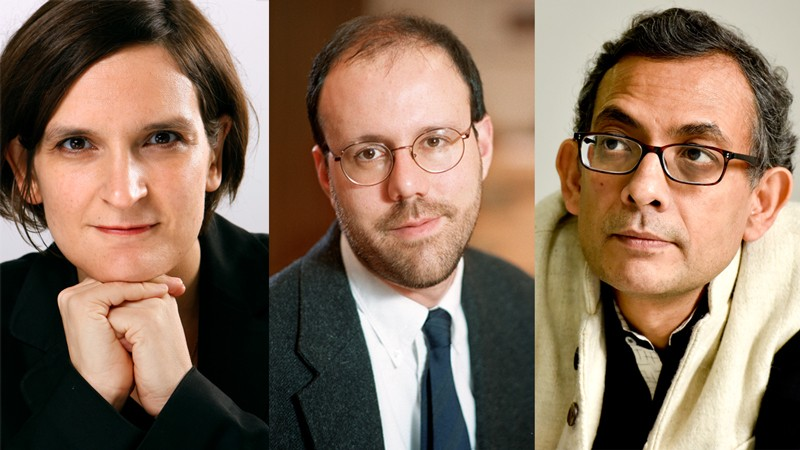
\includegraphics[width=.99\linewidth]{duflo.jpg}
  \caption{Nobel in Economics 2019: Abhijit Banerjee, Esther Duflo, and Michael Kremer}
  \end{figure}
  \end{minipage}
  \hfill
  \begin{minipage}[c]{.30\linewidth}
  \begin{figure}
  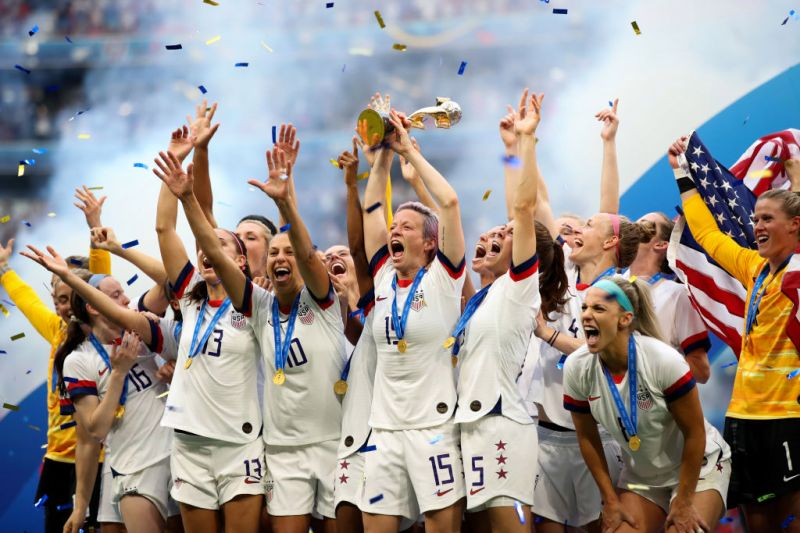
\includegraphics[width=.99\linewidth]{usa-women-team.jpg}
  \caption{US 2019 Women's Soccer team}
  \end{figure}
  \end{minipage}

\normalsize

\pause{}A lot depends on human relations...

\end{frame}

% ------------------------------------------------------------------------------
\begin{frame}

\frametitle{What makes a successful team?}

\begin{figure}
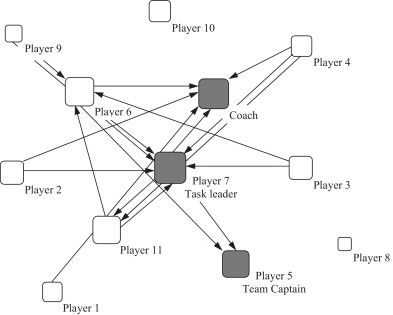
\includegraphics[width=.4\linewidth]{volleyball-team.jpg}
\caption{A volleyball team leadership network (Fransen et al., 2015)}
\end{figure}

\pause{} What processess govern the formation of social networks?


\end{frame}

% ------------------------------------------------------------------------------
% ------------------------------------------------------------------------------
% ------------------------------------------------------------------------------
% ------------------------------------------------------------------------------
% ------------------------------------------------------------------------------

\begin{frame}
\frametitle{Social networks}

\begin{itemize}[<+->]
\item Is it \textit{homophily}, \textit{social balance} (transitivity), \textit{popularity}?
\item Exponential Family Random Graph Models, aka \alert{ERGMs}, can help us.
\item In simple terms, ERGMs allow us to \textit{do}
\begin{quote}
statistical inference on what network patterns/structures/motifs govern social networks
\end{quote}
\end{itemize}

\begin{figure}
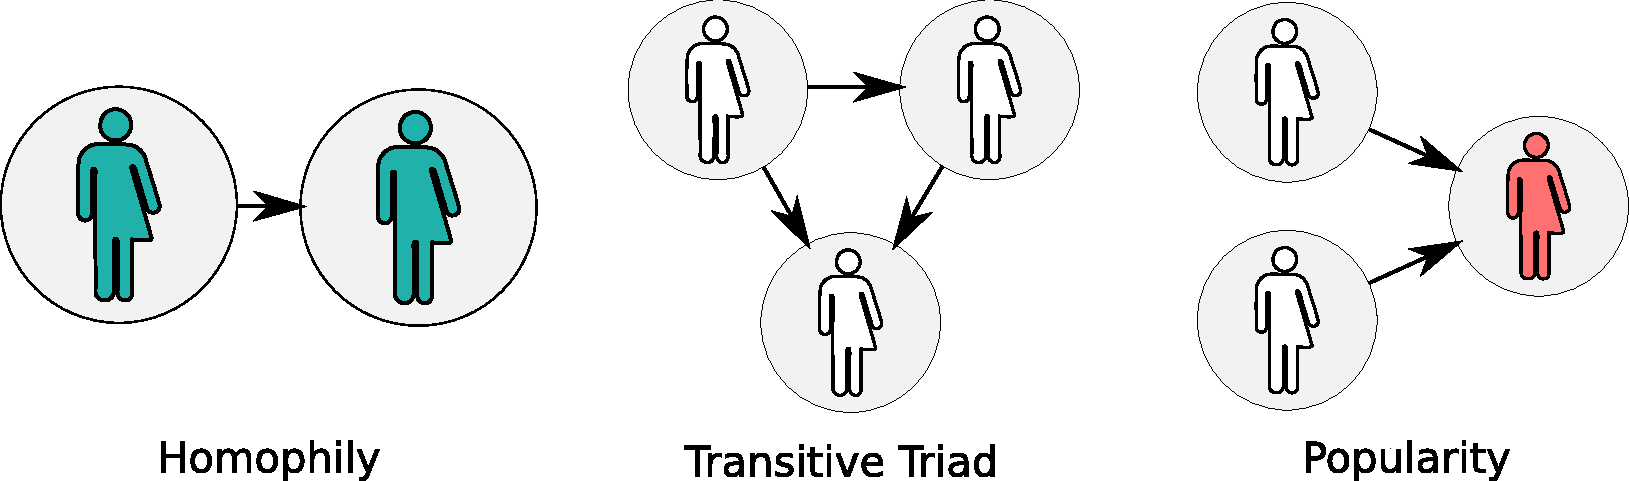
\includegraphics[width=.6\linewidth]{friendly-terms.pdf}
\end{figure}

\end{frame}

% ------------------------------------------------------------------------------
\begin{frame}
\frametitle{Exponential Random Graph Models}

Fairly complex models for studying networks \vspace{1cm}

\begin{minipage}[c]{.55\linewidth}
\begin{figure}
\centering
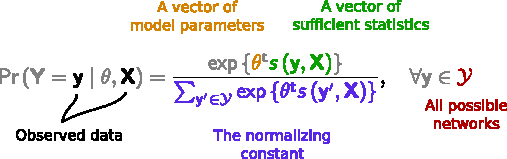
\includegraphics[width=.99\linewidth]{parts-of-ergm.pdf}
\end{figure}
\end{minipage}
\hfill
\begin{minipage}[c]{.40\linewidth}
\begin{figure}
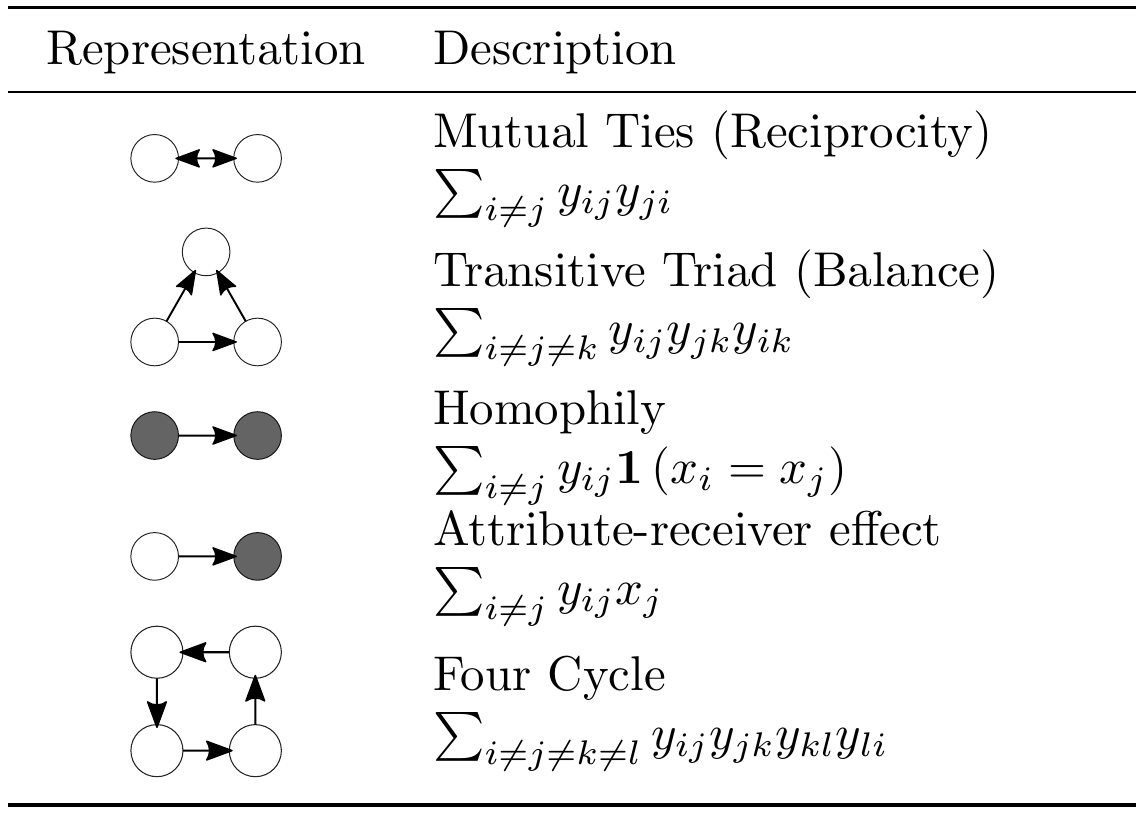
\includegraphics[width=.99\linewidth]{ergm-terms-paper.png}
\end{figure}
\end{minipage}

\vspace{1cm} \pause{} We will be using a novel extension that focuses on small networks (\textbf{ERGMitos})

\end{frame}

% ------------------------------------------------------------------------------
\begin{frame}[label=ergm-vs-ergmito]
\frametitle{ERGMs for small networks}


\begin{figure}
\centering
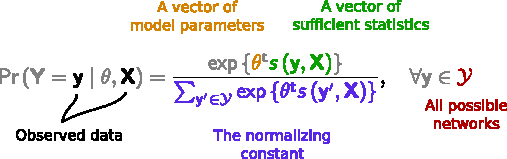
\includegraphics[width=.5\linewidth]{parts-of-ergm.pdf}
\end{figure}\pause{}

Small means that we can calculate the normalizing constant exactly, and thus:\pause{}

\begin{itemize}[<+->]
\item Improved accuracy (bias),
\item Smaller Type I Error rates,
\item Faster estimation (about 20 times faster)
\item A world of possibilities...
\end{itemize}


\vfill

\uncover<6->{(Vega Yon, Salughter and de la Haye (2019))}

\end{frame}

% ------------------------------------------------------------------------------
\begin{frame}[label=examples]

Some results on the emergence of advice-seeking networks in small teams

\vspace{.5cm}

\begin{minipage}{.44\linewidth}
\uncover<2->{
\begin{enumerate}[<+->]
\item Higher Social Perceptiveness \textit{means} more connections.
\item The friend of my friend is my friend.
\item Women ask for advice.
\end{enumerate}
}
\end{minipage}
\hfill
\begin{minipage}{.55\linewidth}
\begin{figure}
\centering
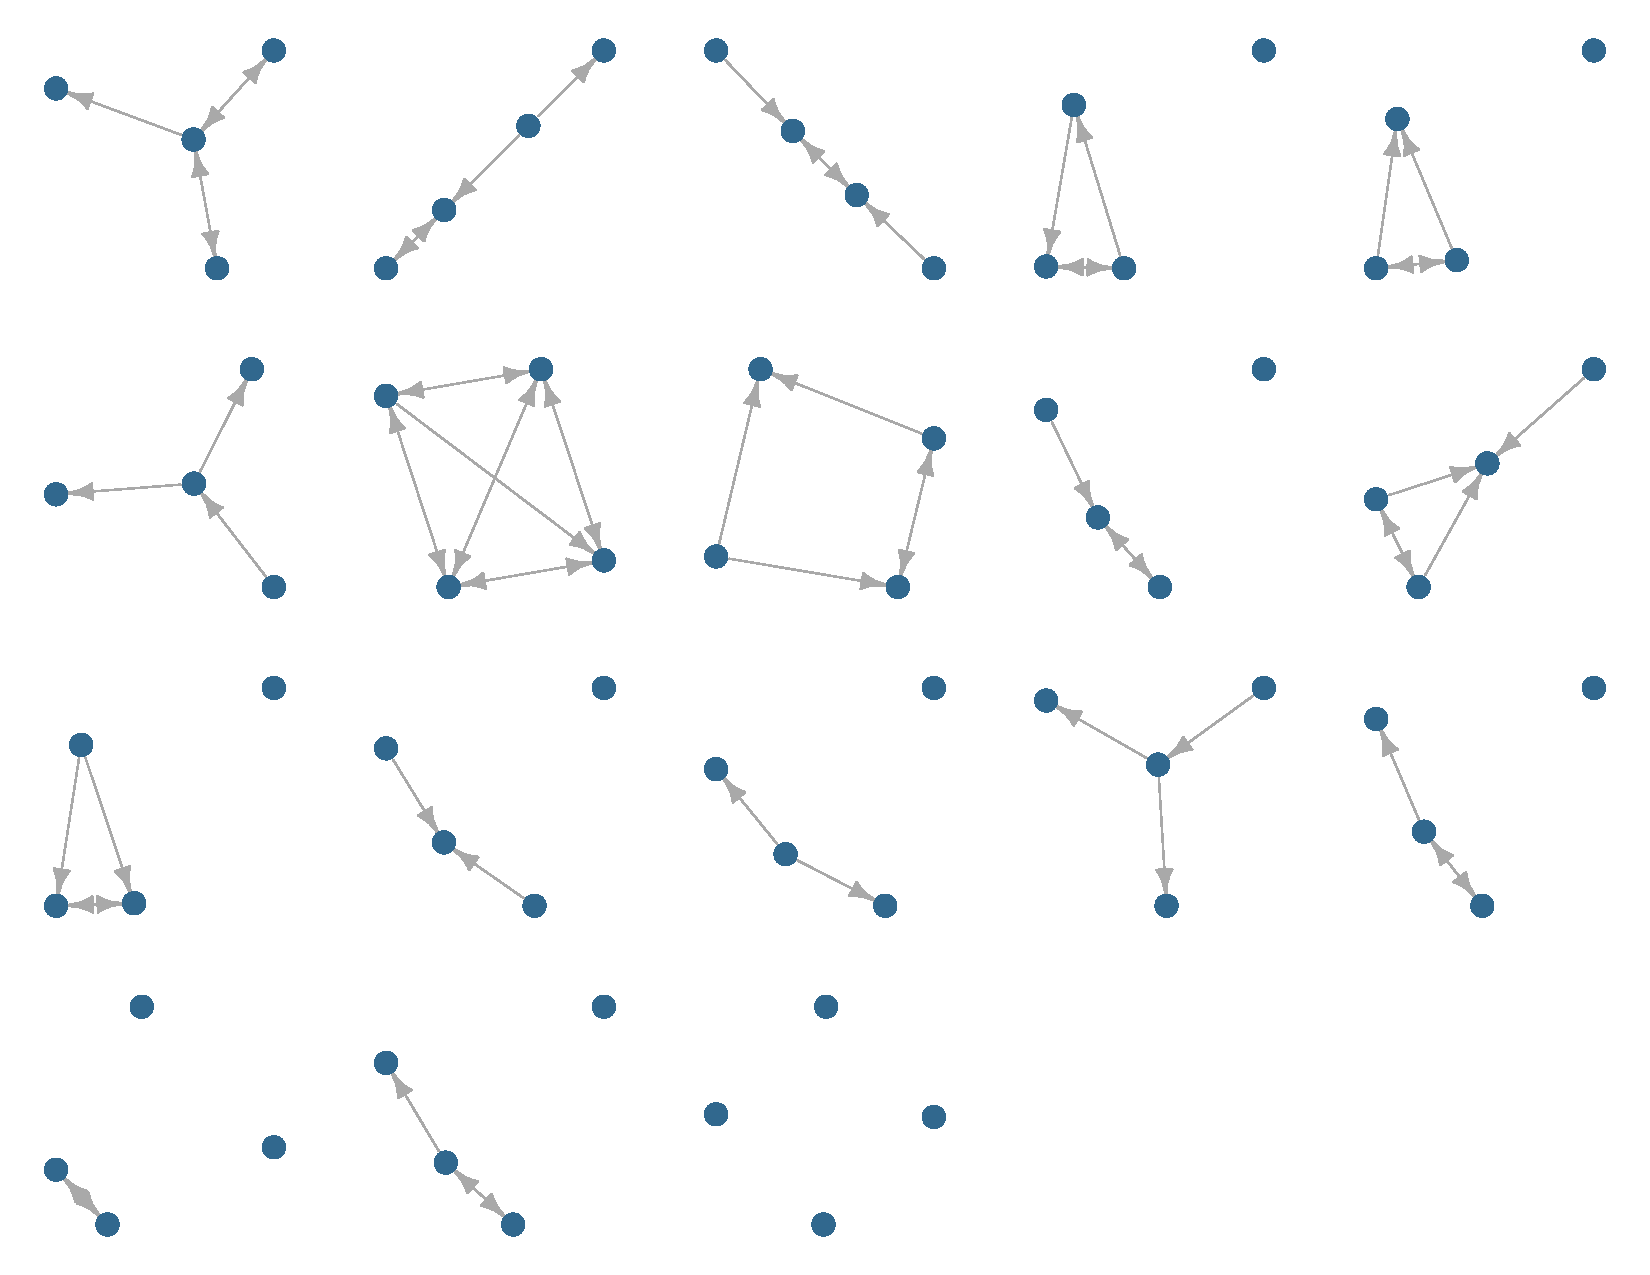
\includegraphics[width = .95\linewidth]{fig/plot-graph-4-1.pdf}
\caption{Advice seeking networks observed in an experiment.}
\end{figure}
\end{minipage}
\end{frame}

\begin{frame}
\frametitle{Concluding remarks}

\begin{itemize}[<+->]
\item The whole is not the sum of the parts
\item Understanding local-macro dependencies is key.
\item We can use ERGMitos to elucidate the processes that govern small networks.
\item Insight into \textbf{team networks} is valuable for understanding team \textbf{process and performance}, and improving \textbf{team design}
\end{itemize}

\end{frame}


% % ------------------------------------------------------------------------------
% \section{Future research}
% \begin{frame}[t]
% \frametitle{Future Research}
% 
% {\bf Goodness-of-fit}\pause
% \begin{itemize}
% \item Is something that will need to be addressed at some point.\pause
% \item The problem is not easy as we need to deal a discrete distribution.\pause
% \item Two key questions: What sufficient statistic to look at? what test?
% \end{itemize}
% 
% \pause {\bf ERGMs for large networks} \pause
% \begin{itemize}
% \item There is still no standard way to estimate ERGMs for large networks.\pause
% \item Most attempts are still depending on simulation methods.\pause
% \item We could use the Snowball Sampling framework together with ERGMitos.\pause{}
% (... I would call this ERGMote)
% \end{itemize}
% 
% \end{frame}



% % ------------------------------------------------------------------------------
\begin{frame}
\maketitle
\begin{center}
\scalebox{2}{\textcolor{uscgold}{Thanks!}}
\end{center}
\end{frame}


\end{document}

